\newpage

\subsubsection{Making Racket more Portable with Linklets}

As described in \secref{sec:intro}, part of the effort of targeting a
new run-time for Racket was making it more portable by separating the
parts that are essential for hosting Racket from the run-time
implementation. \figref{fig:racket-portable} summarizes how different
parts fit together. In the previous versions of Racket, each segment
of the leftmost figure was in C. The first step was to port the
expander from C to Racket, as the Racket expander implements most of
the essential parts for the front-end such as the module system, macro
system, read, expand etc. Given a source program in Racket, the
expander elaborates the code into a core language (that is described
in the previous section) in the form of a bundle of linklets for the
hosting compiler to consume. In other words, linklets essentially make
it possible for the separated segments such as the expander to
communicate with the underlying run-time.

\begin{figure}[h]
  \centering
  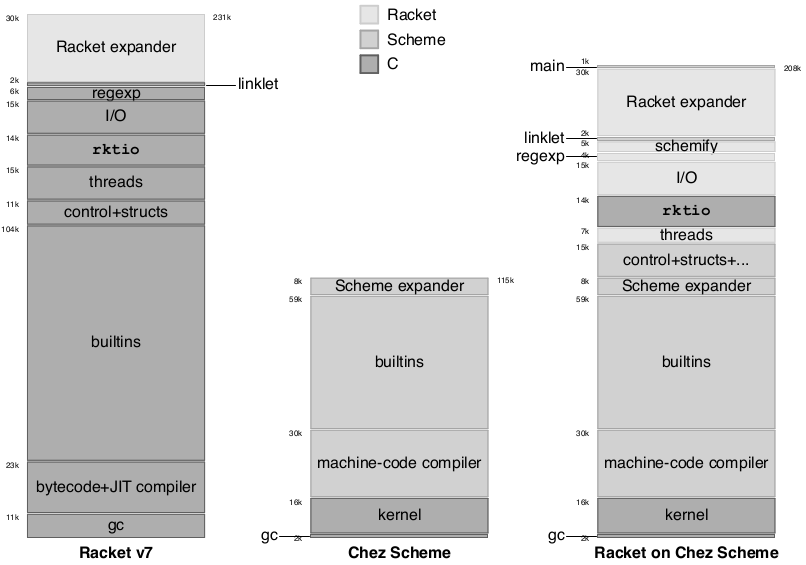
\includegraphics[scale=0.4]{img/racket-portable}
  \caption{Figure used from \cite{racket-on-chez-19}}
  \label{fig:racket-portable}
\end{figure}

The process starts with running the expander offline over itself as
input, outputting a bundle of linklets implementing the expander
itself that the run-time can consume. This bundle is called the
\emph{bootstrapping linklets}. A hosting compiler that implements a
thin API layer for the linklets (the \emph{linklets} layer in
\figref{fig:racket-portable}) can then consume these bootstrapping
linklets to load the essential functionalities into its run-time to
read, expand and evaluate any given Racket code.


show an example where a Racket module is expanded into a linklet
bundle

show an example of the internals of toplevel repl
